\subsection{System and Visualization Design}

\TODO{reviewer 3:
Look at the order of the figures, they do not appear in the same order as they appear in the
text. Also, they are not as close as possible to the reference in the text.
}

We describe the design of \lviz{}, a system for visualizing Windows system
traces.
% \footnote{
% \lviz{} has a number of visualizations. In this paper, we focus on the \VDP{}
% visualization.
% }
We emphasize that the visualization proposed
is not specific to Windows.

\subsubsection{System Traces}
\label{sec:systrace}

Our objective is to visualize detailed system traces.
In the rest of the paper, we will shorten system trace to simply trace.
Our traces are obtained with an enhanced version of
WinResMon~\cite{winresmon} which
captures all operations performed by the Windows kernel
from all processes.
% Our aim is to capture the relevant operations which can be attributed
% to interactions between software (system and applications).
% Collecting trace events in Windows is much harder than UNIX.
% Windows NT (Server 2000, XP, Server 2003, Vista) is a microkernel
% based operating systems.
% Programs are usually written for the Win32 API but those are decomposed
% into microkernel operations.
% However, as Windows is closed source,
% only the Win32 API is documented and not the microkernel API.
% We use WinResMon~\cite{winresmon} to capture system trace.

A WinResMon Windows trace consists of four classes of events
due to operations on processes, files, network and the registry.
An event contains the following properties: (the example events
in Fig. \ref{fig:logex} use the ordering below)
\begin{itemize}
\item {\bf PID/TID} is the ID of the process/thread which 
performs the operation.
%Since it is reusable, it is not unique over time.
\item {\bf Program name} is the pathname of the program binary.
%\item {\bf Group name and User name} is the owner of the process.
\item {\bf Group} and {\bf User name} of the process.
%Unlike UNIX, in Windows there are multiple privileged users. 
% where root is the only privileged user,
% in Windows there are more than one privileged user, such as
% ``{\tt NT AUTHORITY\BS SYSTEM}'',
% ``{\tt NT AUTHORITY\BS LOCAL SERVICE}'',
% ``{\tt NT AUTHORITY\BS NETWORK SERVICE}''
% and arbitrary number of administrators.
\item {\bf Start and end times} of the event.
% are 64-bit timestamps derived from the Intel processor performance counters.
% % are 64-bit timestamps generated by the RDTSC~\cite{rdtsc} instruction.
% % \TODO{This timestamp is a relative timestamp counting from CPU reset.
% % CPU reset may be triggered by system boot or waking up from hibernate,
% % thus one has to add addition bits to ensure monotone increasing timestamp.}
% \TODO{usenix comm:
% A minor technical tidbit: in Sec. 3.1 it is said that start and end time of
% the event is recorded using CPU perf counters; what happens in SMPs? How is
% the timestamp decided?}
\item {\bf Operation type} is specific to the event.
Some examples are given below.
\item {\bf Operation parameters}: The semantics depends on the operation type,
e.g.  resource pathname, file access flags, etc.
% and I/O data.
%Collecting I/O data can be turned on/off by command line options,
%as it is comparably expensive.
%The maximum size of I/O data can also be adjusted.
\item {\bf Return value} from the operation
is either success or an error number explaining why the operation failed.
\item {\bf Call stack trace} of the process which generated the event.
In this paper, we use the deepest function call 
from the corresponding executable, i.e. 
excluding functions in libraries,
but one could also use the full stack trace.
This information is useful to associate a program point in the
application code with the event.
\end{itemize}

% There are 46 operation types in total, 6 related to file,
% 7 related to registry, 5 related to process, and 28 related to network.
Examples of events are file operations, 
e.g.  file\_create, file\_close and file\_read;
registry operations, e.g. reg\_setvalue;
process operations, e.g.  thread\_create;
and network operations, e.g. socket\_bind.
Pathnames of files and registry keys are recorded as operation parameters.
Additional information depending on the specific operation is also recorded.
For example, file\_create, which represents both opening an existing file
and creating a new file, the operation parameters include the pathname of
the opened or created file, access flags, file attributes, creation disposition
(create new, open existing, 
% truncate existing, or append to existing files), 
etc.) and other Windows OS specific information. 
Fig.~\ref{fig:logex} shows two examples of events.
WinResMon can optionally capture the data associated with an
event. (see Sec. \ref{sec:wbbench} which uses network packet data)
% While file and registry resources are represented as paths,
% network resources are represented as network address, i.e. IP address and port.
% Only TCP and UDP protocols are recorded.
% A socket is not associated with an address until {\tt bind()} or {\tt connect()} is called,
% Thus not all network operations are associated with resources.

\begin{figure}
\fbox{\parbox{0.95\columnwidth}{
\tt\tiny
1268 1732
"C:\BS WINDOWS\BS System32\BS svchost.exe" "NT AUTHORITY\BS SYSTEM"
1098307213586 1098307319878
file\_create
"\BS Device\BS HarddiskVolume1\BS WINDOWS\BS Prefetch\BS NET1.EXE-029B9DB4.pf"
access=0x120089, share=0x0, attr=0x0, cd=0x1, co=0x60, si=0x1
STATUS\_SUCCESS
\vspace*{1mm}

\hrule
\vspace*{1mm}

204 960
"C:\BS WINDOWS\BS system32\BS cmd.exe" "GROUP\BS USER"
1101551207684 1101551216008
reg\_queryvalue
"\BS Registry\BS Machine\BS Software\BS Policies\BS Microsoft\BS Windows\BS Safer\BS CodeIdentifiers"
handle=0x78, name="LogFileName", t=0x0, l=0
STATUS\_OBJECT\_NAME\_NOT\_FOUND
}}
%\caption{Two examples of events (without call stack trace)}
\caption{Two examples of events}
\label{fig:logex}
\end{figure}

% A system trace is stored in a compressed text file, where each line 
% records an event.
% We choose this format because it makes filtering and processing easy through
% existing UNIX stream text processing programs.
% The drawback of text file is the difficulty in random accessing,
% however, our visualization programs are implemented to sequentially 
% access the trace.

\TODO{reviewer 3:
The list in section 3.1 can be compressed and figure 1 can be given inline.
}

\subsubsection{Trace Visualization}
\label{sec:vis}

Visualizations for traces need to be able to compress a lot of detail
and yet be usable for illustrating many different
kinds of system behavior ranging from understanding
system administration to debugging to performance evaluation.
% investigating security issues, comparing behavior of program versions, etc.
In order to meet such a wide range of needs, we will see that the visualization
should be adaptable and configurable to show specific aspects for a
given purpose.  It must also be able to scale at different detail levels.

% We describe the design and rationale
% of two novel visualizations: RTG and Extended DotPlot.
% They have different purposes and complement each other.
% Both visualizations are meant for interactive use for exploring different
% ways of looking at the same trace under different visualization
% configurations and zoom levels.
% % modes which also includes
% % interactive zooms to see finer detail.

\TODO{rewritten}
Our visualizations use color for greater visual
bandwidth as well as customization flexibility. 
We support both RGB and CMY color modes.
The RGB color mode displays events on a black background
and is appropriate if the visualization is displayed on monitors to 
make it easy to see events.
For printed output, a CMY mode, which uses subtractive color,
tends to be easier to see.
In this paper, being in print format, we use the CMY mode
and try to minimize the use of yellow due to its closeness to white.
% \footnote{
% % (In \lviz{} switching between RGB and CMY
% % gives RGB:white $\mapsto$ CMY:black, RGB:red $\mapsto$ CMY:cyan, etc.)
% % In this paper, all figures and illustrations use the CMY color model,
% In CMY, the primitive colors are $cyan$, $magenta$ and $yellow$,
% and the composition rules are:
% $cyan+magenta=blue$;
% $cyan+yellow=green$;
% $magenta+yellow=red$; and
% $cyan+magenta+yellow=black$.
% }
% When referring to specific colors generated in
% a visualization, we may specify the color model to
% avoid confusion, e.g. CMY:yellow.
% The RGB color model is better for showing
% detail since it's easier to see color
% pixels on black than it is to see light color print on white paper.
% Since color in RGB is additive,
% it is also more intuitive for reasoning.
% % and the processing algorithms in \lviz{} mainly employ 24-bit RGB.
%We highlight that the reader can see
%more detail in the PDFs by zooming in.


% \TODO{
% eurosys comments:
% It is a bit confusing that DotPlots are presented as normally having white
% for matches, but it seems that in your approach there are colors for
% matches.  Perhaps this should be explained more explicitly.
% }

A {\em binary DotPlot} is a black \& white image
where each axis denotes a sequence of events.
The color of a dot (or pixel) at position ($i$,$j$) is black
when the two events at position $i$ and $j$ from the corresponding sequence
match, and white otherwise.
%\footnote{
%As the print figures are on paper, the CMY mode uses black for a match
%and white for the background. This would be reversed in RGB mode.
%}
The rationale for a binary DotPlot is to visualize event similarity
between two sequences.
It has been used for comparing DNA sequences \cite{dnadp},
visualizing the structure of music \cite{audio}
and investigating data formats and binaries \cite{doxpara}.
DotPlots can be used to do self-comparison
by comparing a sequence with itself or to compare
two different sequences.

\begin{figure}[tb]
\begin{center}
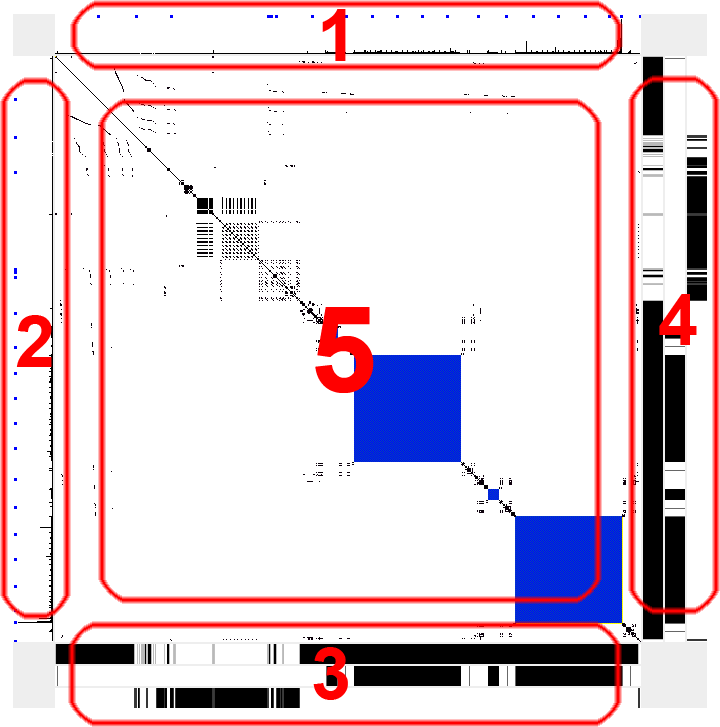
\includegraphics[width=0.5\columnwidth]{dep-elements.png}
\caption{Elements of \VDP{}: axis histograms (Region 1,2);
barcodes (3,4); and extended DotPlot (5). This figure is same as
Fig.~\ref{fig:cp-xcopy} with the added annotation.}
\label{fig:elements}
\end{center}
\end{figure}

Here, we develop a novel DotPlot based visualization which is
extensible and can be configured for many uses.
Our visualization, which we call {\em \VDP{}},
consists of a number of sub-visualizations:
an {\em extended DotPlot} (or simply, DP in the rest of the paper), two
Axis Histograms, and some barcodes.
% We now describe the elements of \VDP{}.
Fig.~\ref{fig:elements} gives an overview of all the elements:
$(i)$ the DP (region 5);
$(ii)$ the x-axis histogram (region 1) and
y-axis histogram (region 2);
and $(iii)$ the x-axis barcodes (region 3) and
y-axis barcodes (region 4).
A larger diagram of the same visualization highlighting various
details is in Fig.~\ref{fig:cp-xcopy}.

An important aspect of the \VDP{} is that it is intended to 
be extensively customizable. Thus, it gives rise to a family of visualizations.
In Sec. \ref{sec:study}, we show how to apply and customize
the \VDP{} for different purposes. The elements of a \VDP{} as follows.

{\bf DP}:
% We overload the DotPlot (DP) to refer either to our
% entire DotPlot visualization or to the extended DotPlot graphic.
Our DP visualization extends a binary DotPlot in a number of ways.
Since a trace can be long, several events are aggregated 
together into a single pixel in a window.
DotPlots which contains aggregated events are drawn as grayscale images
which are then colored using the DP coloring rules for customizing
the appearance.
Normalization or histogram equalization (see Sec.~\ref{sec:imp})
is applied on the image so that the color intensity fits in a displayable range.
Our extended DotPlots (see region 5 in the center of Fig.~\ref{fig:elements})
can be drawn with event-ordering, time-ordering or time-duration-ordering.
In an {\em event-ordered} DP, the events are plotted in
sequence as they occur in the trace.
In a {\em time-ordered} DP, the events are plotted in time order
according to the start time of the event.
Furthermore, each pixel in the visualization can contain several events
as there may be many events occurring close to each other.
% in start time.
Time-ordering differs from event-ordering in that it can be sparse
and allows empty gap if there are no events in a particular time interval.
Furthermore, in event-ordering,
the number of events in a pixel is constant, whereas
in time-ordering,
some pixels do not contain any event while other pixels may have many events.
In a time-duration-ordered DotPlot, the events are plotted in a similar way
to time-ordering
except that the events will be plotted as a rectangular region
with dimensions corresponding to its duration obtained from
the corresponding events on each axis.
Time-ordering, on the other hand, plots 
an event as a single dot.

{\bf DP Matching Rules}:
Unlike a binary DP, our extended DP can look quite different depending
on how matching and coloring rules are specified.
The DP matching rule specifies whether two events
match. The specification allows for matching on 
the properties of an event, e.g. PID/TID, program name,
operation type, etc. (see Sec.~\ref{sec:systrace})
It essentially allows any combination of information about
the event in the trace.
For example, matching based on {\it program name + operation type + resource name}
will give a different visualization from just matching on resource name alone.

{\bf DP Coloring Rules}:
The DP matching rule is used for defining how a DP matches
an event. Given an event which matches the DP matching rule,
the DP color rule specifies what color to display for that event.
% A DP color rule is applicable if the regular expression in the rule
% matches the event.
There can be multiple DP color rules, we use the first matching
rule and there is also a default color if no earlier rules match.
A binary DotPlot, on the other hand, is only in monochrome.

The visualization can be further customized by specifying the colors so
as to combine multiple colors taking
into account either RGB or CMY color modes.
This gives flexibility to emphasize or hide any kind of information
in the trace.
For example, in the RGB mode, the DP color rules
can specify that events which are
file operations are colored red, 
registry operations to be blue, and network operations to be green.
Note that the DP color rule matches independently of the DP matching rule,
e.g. the DP match can be on operation type while the DP color rule could be
on program name.

When combining colors, it is easier to use a RGB mode which is
more intuitive. However, in this paper, CMY is used on all figures.
One way is to use CMY as 3 orthogonal dimensions which would allow 3 different
properties to be visualized.
For example, a cyan pixel in a DP could mean
the events all have property A and an adjacent magenta pixel 
would be a different property B. 
Intersection or union of properties, e.g. property A and B,
allows cyan and magenta to combine giving blue.
Another way is to simply color properties using custom colors.
Our examples mainly use the first method.

{\bf Barcodes} and {\bf Barcode Coloring Rules}:
The barcode sub-visualization
acts as a one-dimensional ruler for the trace on the associated axis, hence its name.
Region 3 and 4 in Fig.~\ref{fig:elements} show X and Y axis barcodes.
The purpose of the barcodes is to visualize multiple aspects of
the trace and allow that to be correlated to the associated event in the DP.

Barcodes are colored using
barcode coloring rules similar to DP coloring rules.
For example Fig.~\ref{fig:cp-xcopy} (see Sec. \ref{sec:cp})
colors the barcode by resource type.
Multiple barcode coloring rules can be specified.
Since barcodes are useful to show properties of the events,
there can be more than one barcode. Each barcode has its own
set of coloring rules, see Fig. \ref{fig:cp-xcopy} which has 3 different
barcodes stacked on the X and Y axis.
In this paper, we number the barcode from inside (top or left depending
on the axis) to outside, i.e. barcode 1 means the inner most barcode.

{\bf Axis Histograms}:
The axis histogram sub-visualization
serves as another kind of ruler for each of the traces on the X and Y axis,
see region 1 and 2 in Fig.~\ref{fig:elements}, providing
time-event correlation information to the traces.
It consists of 
ticks (small blue square on the outer edge) representing unit time intervals
and an associated histogram.
Ticks are evenly distributed in a time-ordered or time-duration-ordered \VDP{}
but can be irregularly distributed in an event-ordered \VDP{},
since there may be many or few events within a unit time interval.
Closely spaced ticks in an event-ordered \VDP{} mean low event frequency.

The histogram component (see region 1 in Fig.~\ref{fig:cp-xcopy})
is used to visualize the density of events or time 
of the trace.
The histogram in a time-ordered or time-duration \VDP{}
represents the number of aggregated events.
In an event-ordered \VDP{},
it represents the total time taken (recall that an event has start and end
time) on the aggregated events.

\subsubsection{A \VDP{} Example}

\begin{figure}[tb]
\begin{center}
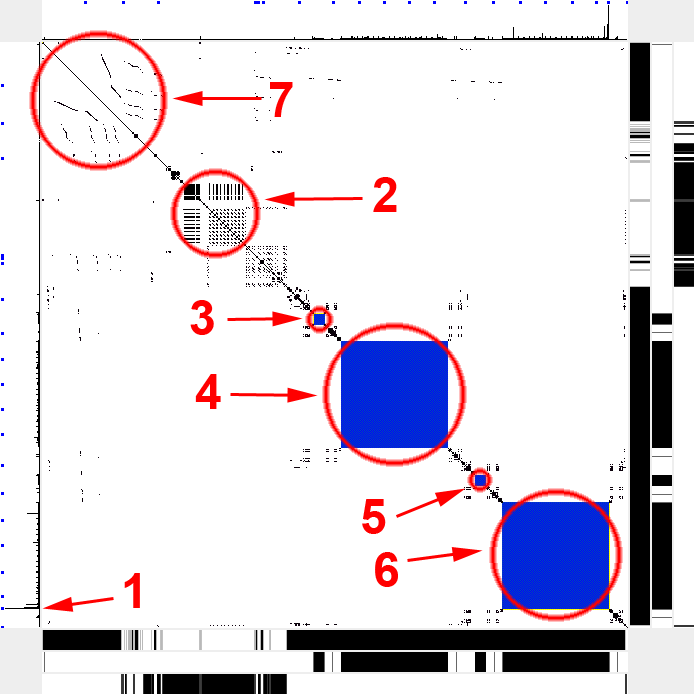
\includegraphics[width=1.0\columnwidth]{dep-cp-xcopy.png}
\caption{Self-comparison event-ordered \VDP{} of {\tt xcopy}
copying 8 files of different sizes with the following configuration rules: 
}
\begin{tabular}{ll}
DP match : & operation + parameter (pathname)\\
DP color : & magenta $\rightarrow$ source; cyan $\rightarrow$ destination;\\
 & black $\rightarrow$ other\\
Bar1 color : & black $\rightarrow$ file operation\\
Bar2 color : & black $\rightarrow$ source/destination files\\
Bar3 color : & black $\rightarrow$ registry operation
\end{tabular}
\label{fig:cp-xcopy}
\end{center}
\end{figure}


\TODO{reviewer 2:
Move figure 4 closer to the text where it is explained (section 3.3) Actually this section is hardly informative. It uses a
lot of forward references so I have to jump all across the paper to see what it really tries to say. I think this section
could be skipped since it does not bring additional value in the discussion at this point.
}

Fig.~\ref{fig:cp-xcopy} illustrates the event-ordered \VDP{}
of a trace of running
\xcopy{} to copy two directories with files of different sizes.
The \VDP{} uses self comparison of the \xcopy{} trace with
the DP matching rule on operation and parameter (resource pathname).
The \VDP{} configuration consisting of a DP ordering, DP matching rule,
DP coloring rules and barcode coloring rules
is given in the caption of the figure.
The non-white regions inside the DP show when \xcopy{} is using the
same resource with the same operation and parameter.
Its color represents the resource.
Each blue square is the aggregated visualization effect from
copying a file (see Sec. \ref{sec:cp}).
The file sizes are apparent from the sizes of the small (region 3 and 5)
and big (region 4 and 6) blue squares.
We can see that file operations are performed at the start (barcode 1),
but those files are neither source nor destination files (barcode 2).
Registry operations are performed relatively
quickly compared to file operations,
because the blue ticks in the histogram above region 2 are spaced further apart
than the blue ticks above region 4 and 6.
Further discussion on this example is in Sec. \ref{sec:cp}.

The DP user interface allows exploration of the trace by zooming in
This allows us to see quite different detail from an aggregated view.
We can see the effects of visualizations at different scales,
Fig.~\ref{fig:cp-xcopy} shows the aggregate behavior which
is a different picture from the magnified view in
Fig.~\ref{fig:cp-zoom} which shows the individual file operations in \xcopy{}.
Zooming creates a new window as one may want to see many different
detail levels at the same time. Clicking inside the DP selects
a pixel to give more details of the events aggregated in that pixel. When
the mode is event-ordering, the events displayed are those events contained
in that pixel. Whereas with time-ordering or time-duration-ordering,
the events are those events which intersect in time with the time interval
represented by that pixel. 

% {Zoom and Click}. 
% Zoom is one of the most important features that we must have.
% The first time the DotPlot is created, it encompases the entire log files
% that may contain hundred of thousands events.
% The pixel shown in this state contains aggregated number of events
% and the color might be seen as the addition of multiple colors.
% Zoom allows us to go deep into a particular region of interest 
% and explore the traces in a more fine grained manner.
% Clicking on the DotPlot area will print out the events
% residing in the clicked region which is very helpful in exploration process.
% 
% 
% We designed our DotPlots UI to implement the above control operations.
% We use an extensive configuration file to specify most of the parameters for the visualization
% and we use command line interface to interact with the UI.
% The static parameters in the configuration file includes:
% list of log files, list of color rules (regex / plain search pattern),
% DotPlot fields selection, DotPlot color rules, Barcode color rules,
% invert color option, gamma correction value, histogram equalization option, etc...

% The command line accepts 4 commands: "dpe" to render a DotPlot Event-Ordering,
% "dpt" is for DotPlot Time-Ordering, "dptd" is for DotPlot Time-Duration-Ordering,
% and "reload" to reload the configuration file.
% 
% A UI frame will pop out when one of the "dpe", "dpt", "dptd" command is put.
% The UI looks like \TODO{Figure ?}
% 
